%
% File: chap03.tex
% Author: Farah Hassan
% Description: Explains experiments which I ran. 
%
\let\textcircled=\pgftextcircled
\chapter{Results}
\label{chap:intro}

\initial{R}ecalling from the Introduction that the aim of this project was to assess whether Bayesian regression can aid in the stress analysis of materials with complex grain structures, this section details the result of fitting challenging simulated X-Ray diffraction strain measurements (detailed in section 3) using Bayesian linear regression in comparison to the fit outcomes yielded by Least-Squares linear regression, the Nuclear industry standard. Emphasis is placed particularly on assessing the:

\begin{itemize}
    \item accuracy of stress tensor estimate relative to the result yielded by Least-Squares regression and in reference to the known stress tensor from which the simulated measurements were generated from,
and \item feasibility of the confidence intervals yielded by the fit relative to how far in reality the fitted stress is from the known true stress.
\end{itemize}

%=======
\section{The Extent of the Prior Distribution's Influence on Fit Outcome}
\label{subsec:subsec01}

\subsection{Changes to the Prior Distribution's Mean}
\label{subsec:subsec01}

Figure 4.1 illustrates the results of a test wherein two simulated strain measurements, with high and low Normally distributed noise, were fit 6 times using Bayesian linear regression with decreasing prior restrictiveness (increasing standard deviation) with the fitted $\sigma_{11}$ tensor plotted in relation to the prior value. It was observed that that if the prior is not restrictive, the fit converged to the value implied by the distribution, suggesting that Bayesian regression favoured the data over the prior knowledge except in cases the certainty in the prior knowledge was high.\\

\begin{figure}[h]
 	\centering
 	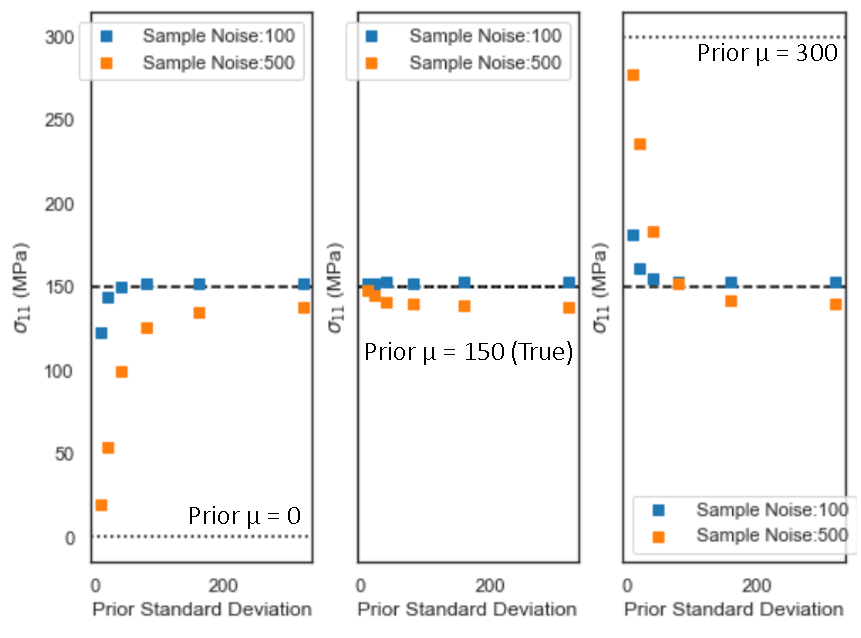
\includegraphics[width=0.8\textwidth]{chapters/chapter03/fig03/prior.png}
 	\mycaption
 	{Plot illustrating the relationship between fitted stress and Bayesian prior strength for two simulated samples of strain measurements, containing high (orange) and low (blue) uncertainties in peak position. As prior strength decreases, the fitted stress tends to the values implied by the measurements.}
    \label{fig:RHP02}
 \end{figure}

Another notable observation was that fit outcomes for measurements with higher uncertainty were more heavily skewed to the value suggested by the prior distribution, although were ultimately overcome by what the measurements implied. For example, in the case where the prior distribution's mean was set to the true stress value (figure 4.1), the fit outcome was closer to the true value, due to the prior distribution's influence on the fit, but ultimately converged to the result implied by the data, which was further away. \\

Importantly, this test allowed for the determination of an appropriate value ($\sigma$ = 200) for the strength of the prior distribution for further testing of simulated measurements with the same true stress value, highlighting the possibility of carrying out similar calibration in industry when using Bayesian regression to enable the selection of an appropriate and bespoke prior strength, which would not skew the fit outcome unnecessarily.\\



\subsection{Changes to the Nature of the Likelihood Function}
\label{subsec:subsec01}

When the likelihood function (see section 2.3) for Bayesian regression is Normal, it is operating on the basis of the same assumptions as Least-Squares regression: that errors are Normally distributed and therefore that the fit outcome is Normally distributed about the true stress value.\cite{a2017_bayesian} This, coupled with a non-restrictive prior distribution, leads to a Bayesian fitted stress that is identical in practice to that yielded by Least-Squares Regression, as illustrated in figure 4.2, a result which was observed consistently. \\

Figure 4.2 illustrates a strain measurement fit using Bayesian regression with a Normal likelihood function and Least Squares regression, the results are indistinguishable for practical purposes.\\

\begin{figure}[h]
 	\centering
 	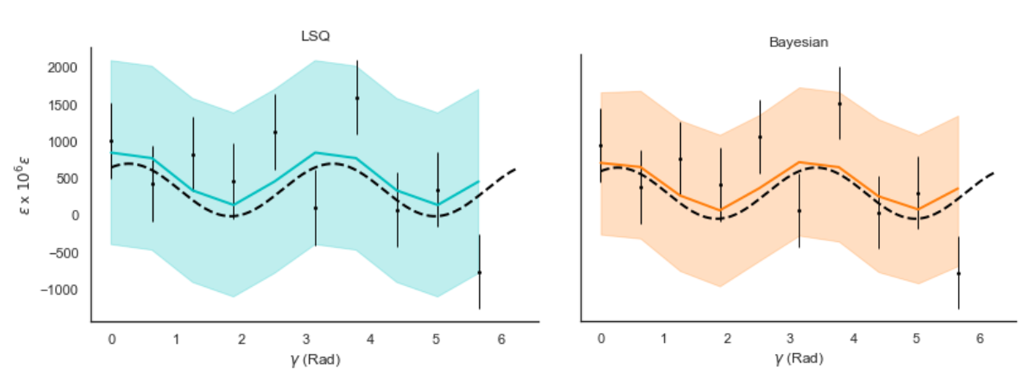
\includegraphics[width=0.9\textwidth]{chapters/chapter03/fig03/samefit.png}
 	\mycaption
 	{A strain measurement fit using Bayesian regression with a Normal likelihood function and Least Squares regression, the results are indistinguishable for practical purposes. Shading indicates 95th percentile and the coloured lines indicate fit outcomes for Least-Sqaures (Blue) and Bayesian (Orange).}
    \label{fig:RHP02}
 \end{figure}

Changing the Likelihood function to a Student's T distribution (see section 2.3) would theoretically make the fit more robust, due to the increased flexibility to outliers caused by the wide tails of the t - distribution, which would allow for more measurements to lie further from the mean. However, this change did not consistently yield a significantly different fit outcome for measurements which contained only Normally distributed errors or only T - distributed errors with 3 degrees of freedom (see sections 4.2 and 4.3 for more detailed analysis of these samples) to that obtained using Least-Squares regression. \\

In the case of samples with a combination of Normally and T-distributed noise with two degrees of freedom, the robust Bayesian yielded a significantly more accurate fit than both Least-Squares and Bayesian Regression, the results of which were equally inaccurate in practice. Analysis for measurements with a combination of Normal and T error distributions is detailed in section 4.4. \\

Figure 4.3 illustrates the Least-Squares fit outcome (used interchangeably hereafter with simple Bayesian regression, wherein the likelihood function is Normal) compared to the robust Bayesian fit outcome for a sample of measurements containing a combination of Normal and Student's T-distributed errors. Importantly, not only is the Least-Squares fit less accurate than the Robust Bayesian fit, it is more certain that the fit is accurate. Furthermore, the ability to observe a potentially bi-modal distribution for the stress tensor components is valuable and makes the confidence intervals more feasible, as the fit is considering the possibility of the outliers being accurate. \\


\begin{figure}[h]
 	\centering
 	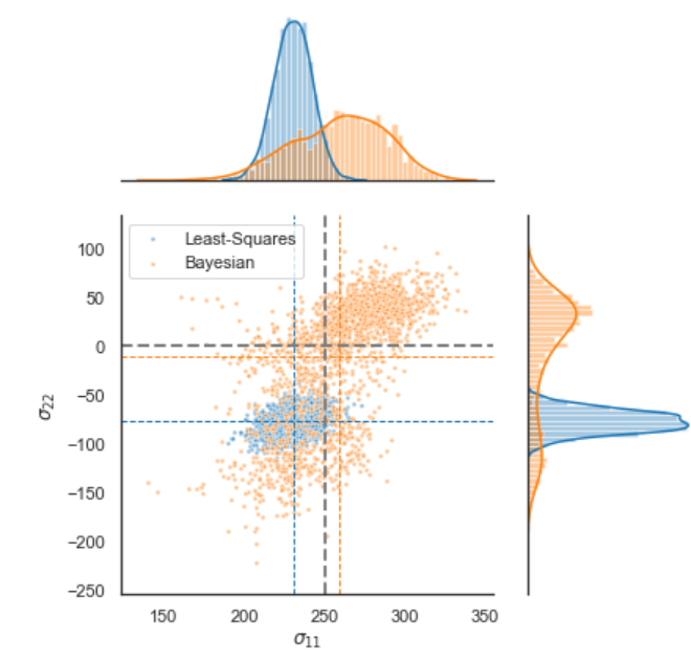
\includegraphics[width=0.8\textwidth]{chapters/chapter03/fig03/supervisor.png}
 	\mycaption
 	{Least-Squares (blue) and robust Bayesian regression (orange) fit outcomes for a sample with both Normally and T - distributed errors. The Least-Squares distribution is further from the true stress (grey) and more certain than the robust Bayesian regression.}
    \label{fig:RHP02}
 \end{figure}




\section{Samples with Normally Distributed Errors}
\label{sec:sec01}

The fit outcomes for robust Bayesian and Least-Squares for samples with only Normally distributed errors, simulating peak position uncertainty, were indistinguishable regardless of  error magnitude, as illustrated in figures 4.4 and 4.5. The robust Bayesian regression failed to generate a more accurate or more representative fit outcome and, While there where small differences in distribution height, slight observed differences were not consistent across different samples and overall the fitted stress tensor components were close in shape and accuracy.

\begin{figure}[H]
 	\centering
 	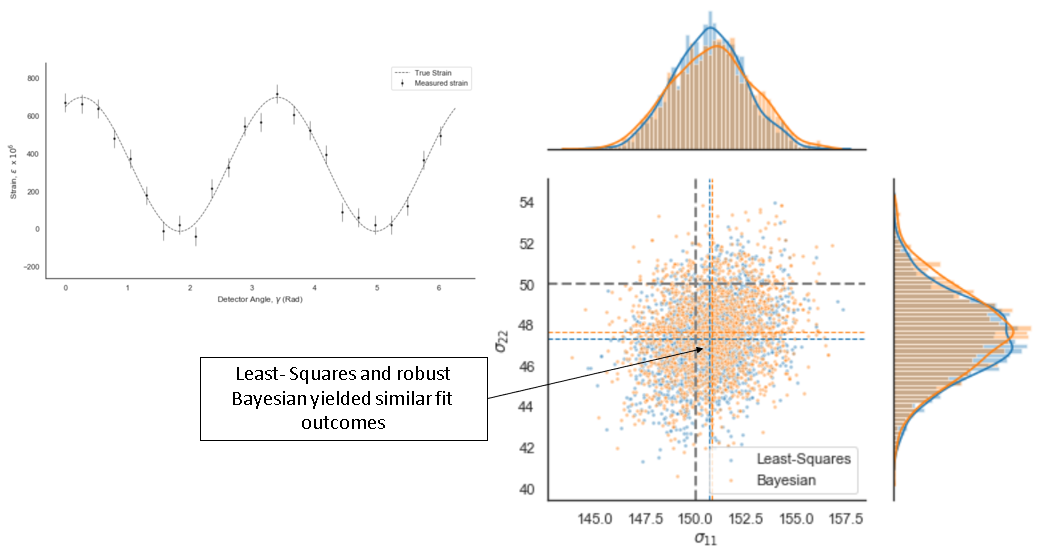
\includegraphics[width=0.9\textwidth]{chapters/chapter03/fig03/s13D.png}
 	\mycaption
 	{Least-Squares (blue) and robust Bayesian regression (orange) fit outcomes for a sample of strain measurements with only Normally distributed errors, simulating low uncertainty in peak location. Both fit outcome means (the dotted lines) are equally far from the true stress (grey) and have similar confidence intervals (indicated by the spreads).}
    \label{fig:RHP02}
 \end{figure}

\begin{figure}[H]
 	\centering
 	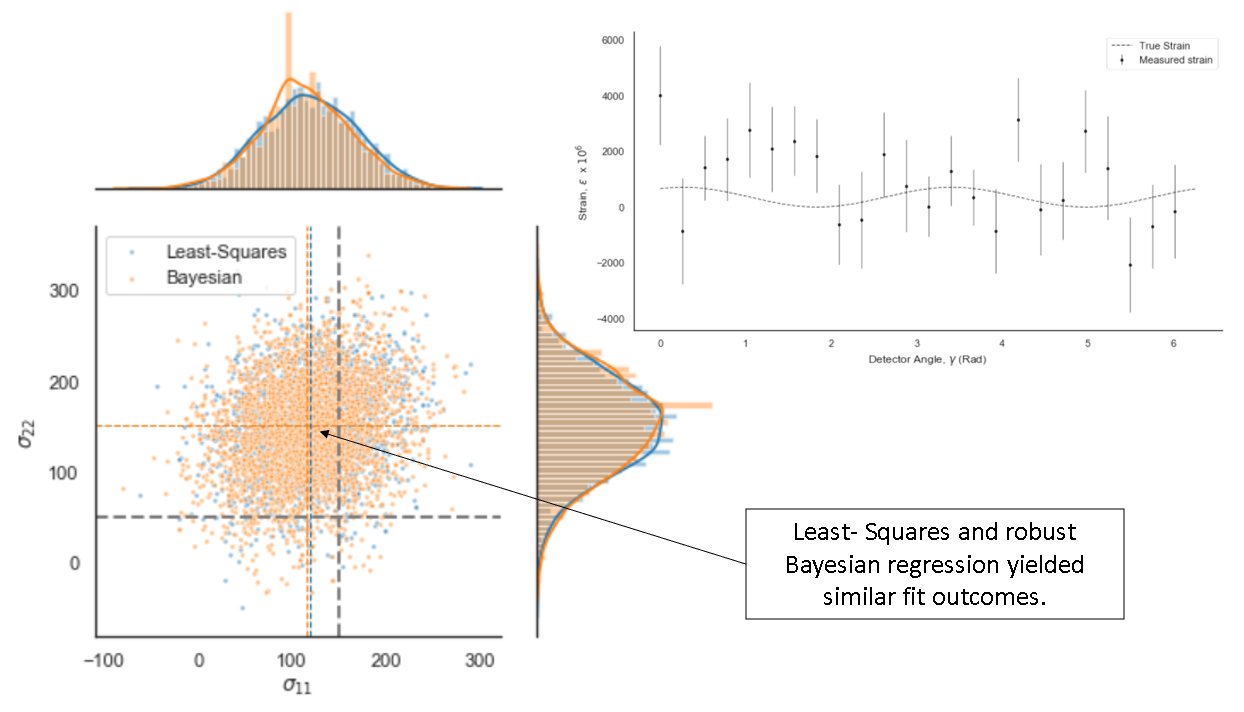
\includegraphics[width=0.9\textwidth]{chapters/chapter03/fig03/s63D.png}
 	\mycaption
 	{Least-Squares (blue) and robust Bayesian regression (orange) fit outcomes for a sample of strain measurements with only Normally distributed errors, simulating high uncertainty in peak location. Both fit outcome means (the dotted lines) are equally far from the true stress (grey) and have similar confidence intervals (indicated by the spreads).}
    \label{fig:RHP02}
 \end{figure}




\section{Simulated Measurements with T- Distributed Errors}
\label{sec:sec01}

As with the measurements which contained only Normally distributed errors, the robust Bayesian regression also failed to yield a more accurate fit outcome for measurements which only contained T - distributed errors, which were simulating the uncertainty associated with grain sampling statistics in X - Ray diffraction measurements.\\

The results, which were that fit outcomes did not differ significantly for Least-Squares and robust Bayesian regression are illustrated in 4.6 \\


\begin{figure}[H]
 	\centering
 	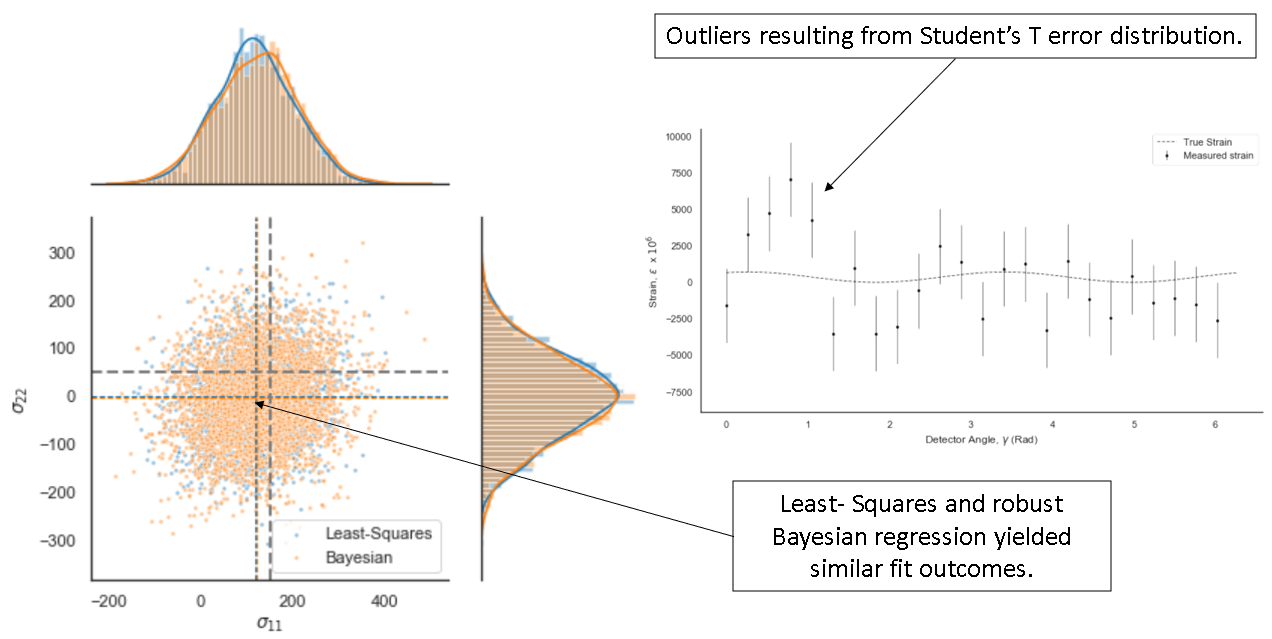
\includegraphics[width=0.9\textwidth]{chapters/chapter03/fig03/s33D.png}
 	\mycaption
 	{Least-Squares (blue) and robust Bayesian regression (orange) fit outcomes for a sample of strain measurements with only T - distributed errors, simulating high uncertainty originating from grain sampling statistics. Both fit outcome means (the dotted lines) are equally far from the true stress (grey) and have similar confidence intervals (indicated by the spreads).}
    \label{fig:RHP02}
 \end{figure}


\section{Simulated Measurements with Manually Introduced Outliers}
\label{sec:sec01}

To generate extreme outliers, simulated strain measurements were created with a combination of Normal and T - distributions (as introduced in section 2.3) with two degrees of freedom. Robust Bayesian consistently outperformed Least-Squares regression for these samples, both in the accuracy of the fitted stress tensors and in the feasibility of the confidence intervals. \\

The results are illustrated using figures 4.7 and 4.8. Importantly, the distribution of stress tensor components yielded by the robust fit is bi-modal in some cases, showing that the outliers were considered as potentially accurate. Furthermore, the stress distribution yielded by the robust Bayesian fit is more scattered, correctly recognising its lack of certainty of the fit outcome caused by the presence of outliers and noise.\\

In contract, the stress distributions yielded by Least-Squares regression were heavily influenced by the outliers, having shifted the fitted distribution to justify their presence to maintain alignment with the assumption that the errors are Normally distributed. Furthermore, the Least-Squares outcome failed to recognise its inaccuracy, incorrectly identifying the fit as quite certain, as seen by the narrow shape of the distribution. In some cases, the fitted stress distribution was so confident of an inaccurate result that the true value of stress tensor components did not lie within it (figure 4.8). 

\begin{figure}[H]
 	\centering
 	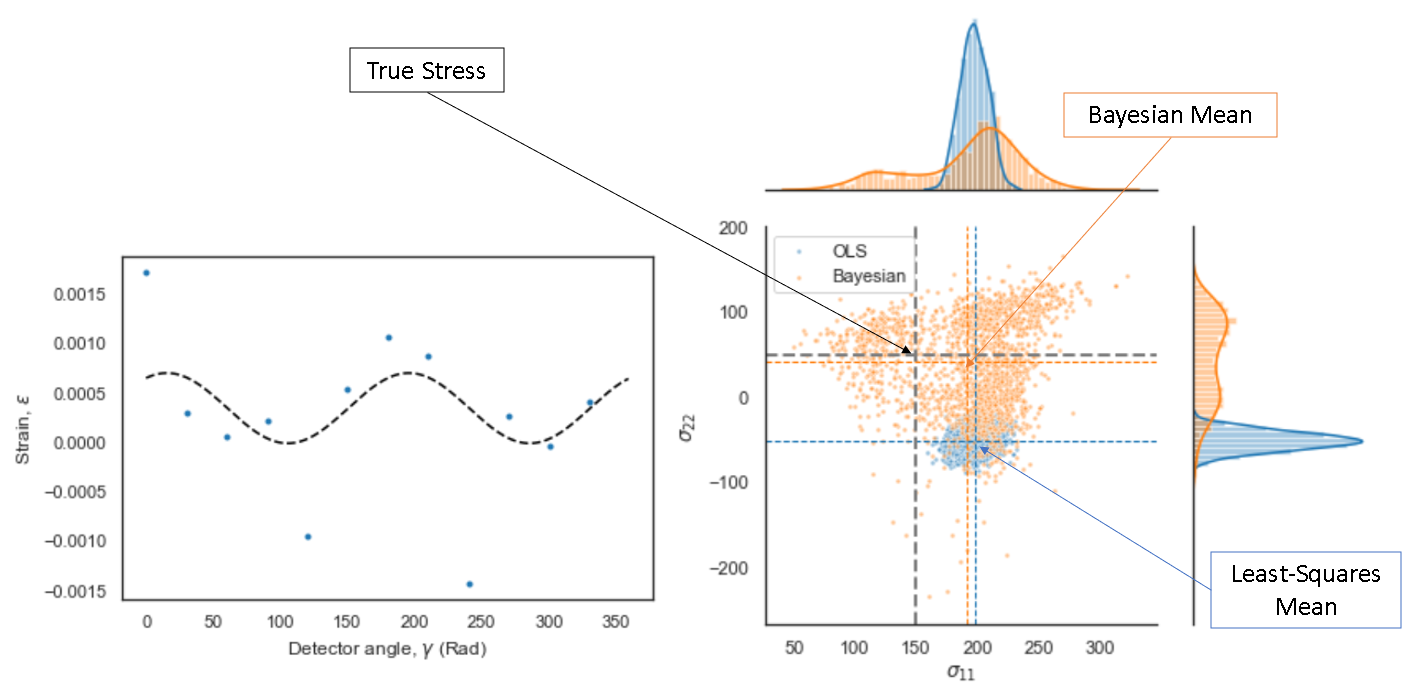
\includegraphics[width=0.9\textwidth]{chapters/chapter03/fig03/s93D.png}
 	\mycaption
 	{Least-Squares (blue) and robust Bayesian regression (orange) fit outcomes for a sample with both Normally and T - distributed errors. The Least-Squares distribution is further from the true stress (grey) and more certain than the robust Bayesian regression.}
    \label{fig:RHP02}
 \end{figure}

\begin{figure}[H]
 	\centering
 	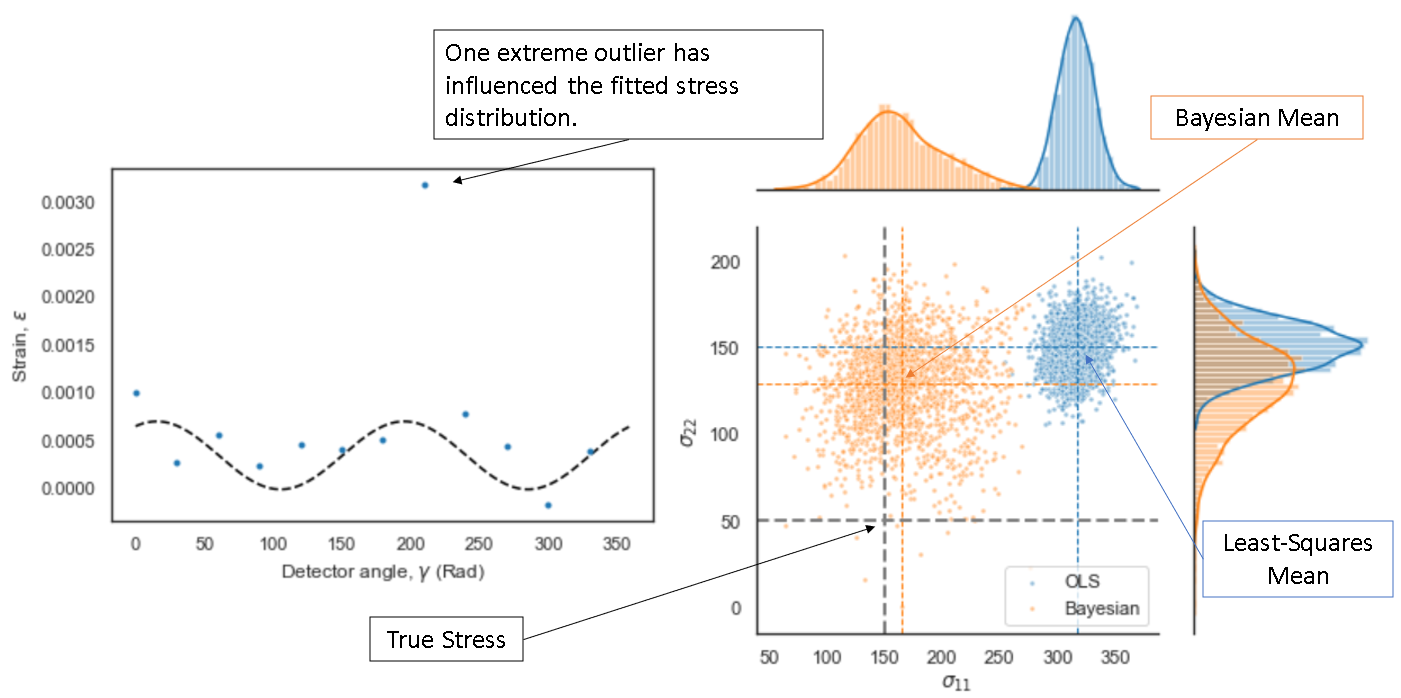
\includegraphics[width=0.9\textwidth]{chapters/chapter03/fig03/s103d.png}
 	\mycaption
 	{Least-Squares (blue) and robust Bayesian regression (orange) fit outcomes for a sample with both Normally and T - distributed errors. The Least-Squares distribution is further from the true stress (grey) and more certain than the robust Bayesian regression. In this case the fit outcome was influenced by one extreme anomaly.}
    \label{fig:RHP02}
 \end{figure}


\section{Outlier Detection Using Bayesian}
\label{sec:sec01}

As described in section 3.2.3, outlier detection was attempted within Bayesian by changing the nature of the Bayesian likelihood distribution to a variation of the Bernoulli distribution (as introduced in section 2.3). The results varied depending on the sample's complexity; for samples with one type of error distribution (Normal or T-distributed only), the fit outcome was not significantly more accurate than either Least-Squared or Robust Bayesian. \\

In simulated measurements with error distributions which were a combination of Normal and Student's T, there were some significant improvements observed. Figure 8 illustrates the fit yielded by the regression using outlier detection of the same sample as in figure 4.7. Although it also yields a bi-modal distribution, as in the case of the robust Bayesian regression, the fit which incorporates the outlier detection correctly identifies the true value as more likely than that implied by the anomalies.

In figure 4.10, the same test was carried out on the sample in figure 4.8, with the result being that the fitted stress outcome of the robust Bayesian with the outlier detection was not significantly more accurate or more representative than the robust regression without the automated outlier detection. 



\newpage
\begin{figure}[h]
 	\centering
 	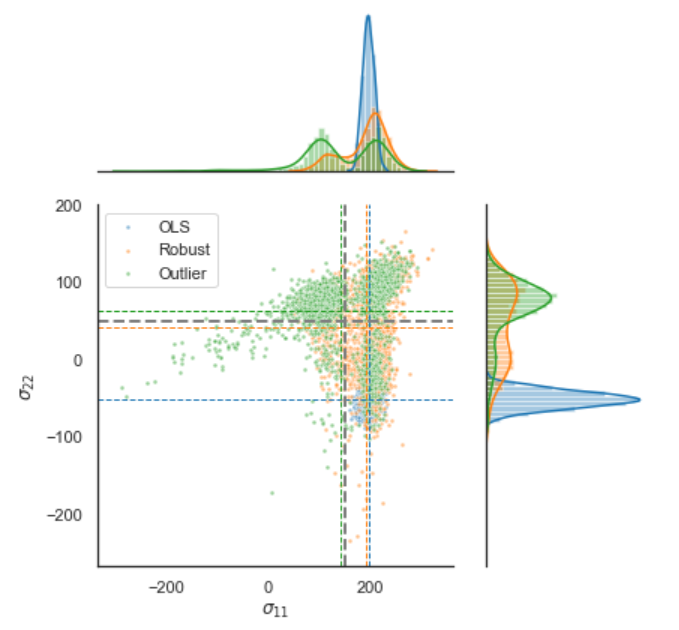
\includegraphics[width=1\textwidth]{chapters/chapter03/fig03/outlierS9.png}
 	\mycaption
 	{Least-Squares (blue), robust Bayesian regression (orange), and Bayesian with outlier detection (green) fit outcomes for a sample with both Normally and T - distributed errors. While robust Bayesian regression with and without outlier detection yields bi-modal distributions, the former correctly identifies the true value of the stress tensor component as being the more probable result.}
    \label{fig:RHP02}
 \end{figure}
\newpage
\begin{figure}[H]
 	\centering
 	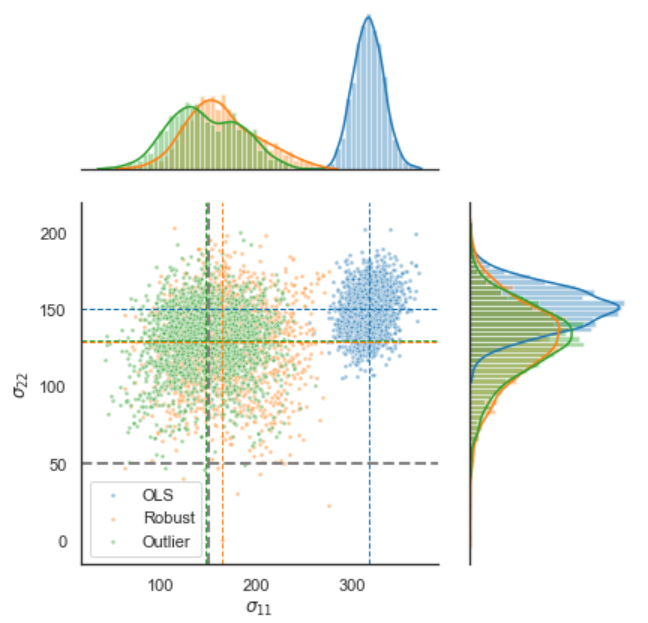
\includegraphics[width=1\textwidth]{chapters/chapter03/fig03/outlierS10.png}
 	\mycaption
 	{Least-Squares (blue), robust Bayesian regression (orange), and Bayesian with outlier detection (green) fit outcomes for a sample with both Normally and T - distributed errors. The fit distribution for Bayesian with and without outlier detection are similar for this sample.}
    \label{fig:RHP02}
 \end{figure}
